\section{Results}
\label{sec:Results}
% Chaos
From figure \ref{fig:Contour} (see also figure \ref{fig:AllProbabilities} in the Online Appendix) we conclude that, in our model, the likelihood of chaotic dynamics reaches an optimum for near-neutral competition at the prey level. This result remains true for systems with a different number of species. The likelihood of chaos also increases with the size of the food web. This effect should not be surprising: the more dimensions the phase space has, the easier is to fulfill the requirements of the complex geometry of a chaotic attractor \citep{Strogatz1994}. Even in those higher dimensional cases, there is still a clear maximum at near-neutral competition. The probability of chaos shows another local, lower maximum for weak competition coupling, while stable solutions are very rare (figure \ref{fig:Biodiversity}.A). Possibly due to the weaker coupling we get less phase locking of the predator prey cycles in this case.

\begin{figure}
	\begin{center}
		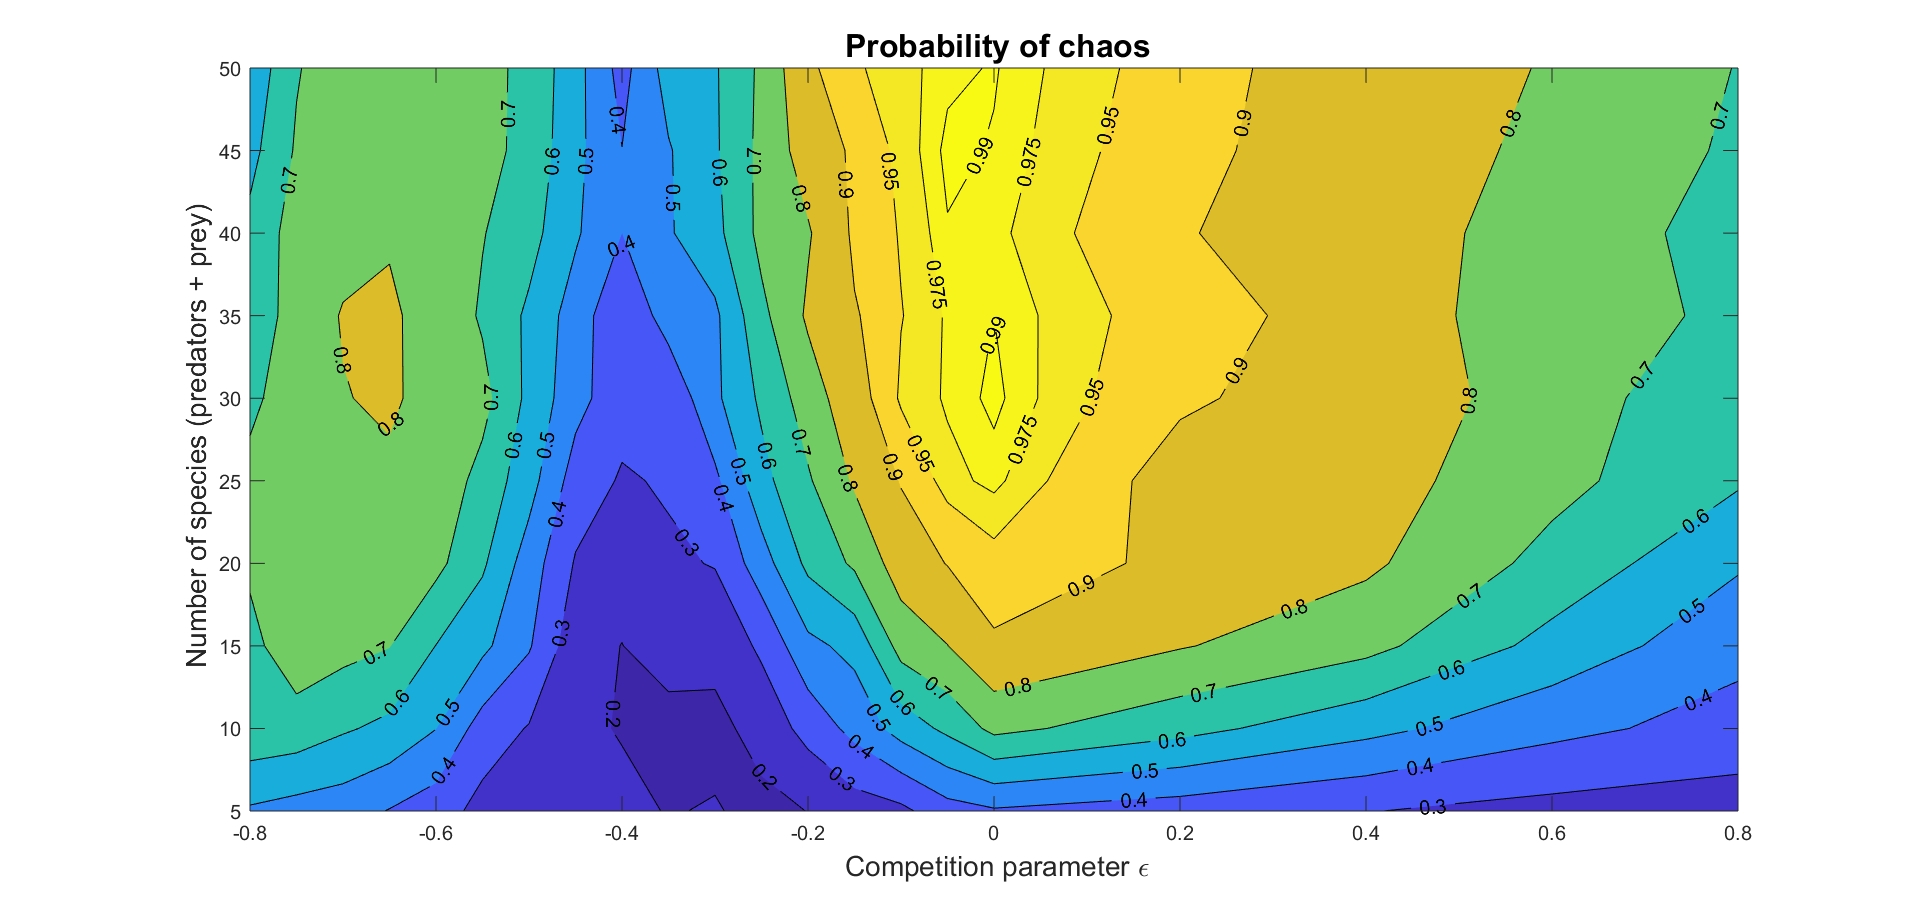
\includegraphics[width=1\columnwidth]{contour.png}
	\end{center}
	\caption{Contour map showing the probability of chaos for various competition parameters (horizontal axis) and number of species (vertical axis). The consumers' population is fixed as $ 2/3 $ of the prey's population. Notice that chaotic attractors appear more easily (i.e., for smaller systems) the closer is the competition to neutral (i.e., $ \epsilon = 0 $).}
	\label{fig:Contour}
\end{figure}

% Biodiversity
As expected, we also found a clear relationship between the probability of chaos and the biodiversity. In all our cases the diversity of chaotic dynamics were highest (figures \ref{fig:Biodiversity} B,C) and the overall diversity peaked approximately at the near-neutral situation. Interestingly also the cyclic solutions were clearly much more diverse than cases with stable dynamics (figures \ref{fig:Biodiversity} B,C). In fact the difference in biodiversity of the situation with chaos and cycles was rather small (figure \ref{fig:Biodiversity}.C). This conclusion remains true for food webs of different sizes (figure \ref{fig:BiodBoxAndWhisker} in the Online Appendix). From figure \ref{fig:Biodiversity}.D, we see that the prey biomass remains relatively stable for the whole range of competition parameters, with the exception of weak interspecific competition, where it reaches a maximum. The predator biomass grows almost linearly as the competition moves leftwards, from near-neutral to strong intraspecific, while the prey biomass remains constant. We think this can be understood from the effect of niche complementarity which causes effectively an increase in the total prey biomass. Like in a two-species model this increase in prey biomass results in an increase of predator biomass only (cf. \citet{Rosenzweig1963}).

\begin{figure}
	\begin{center}
		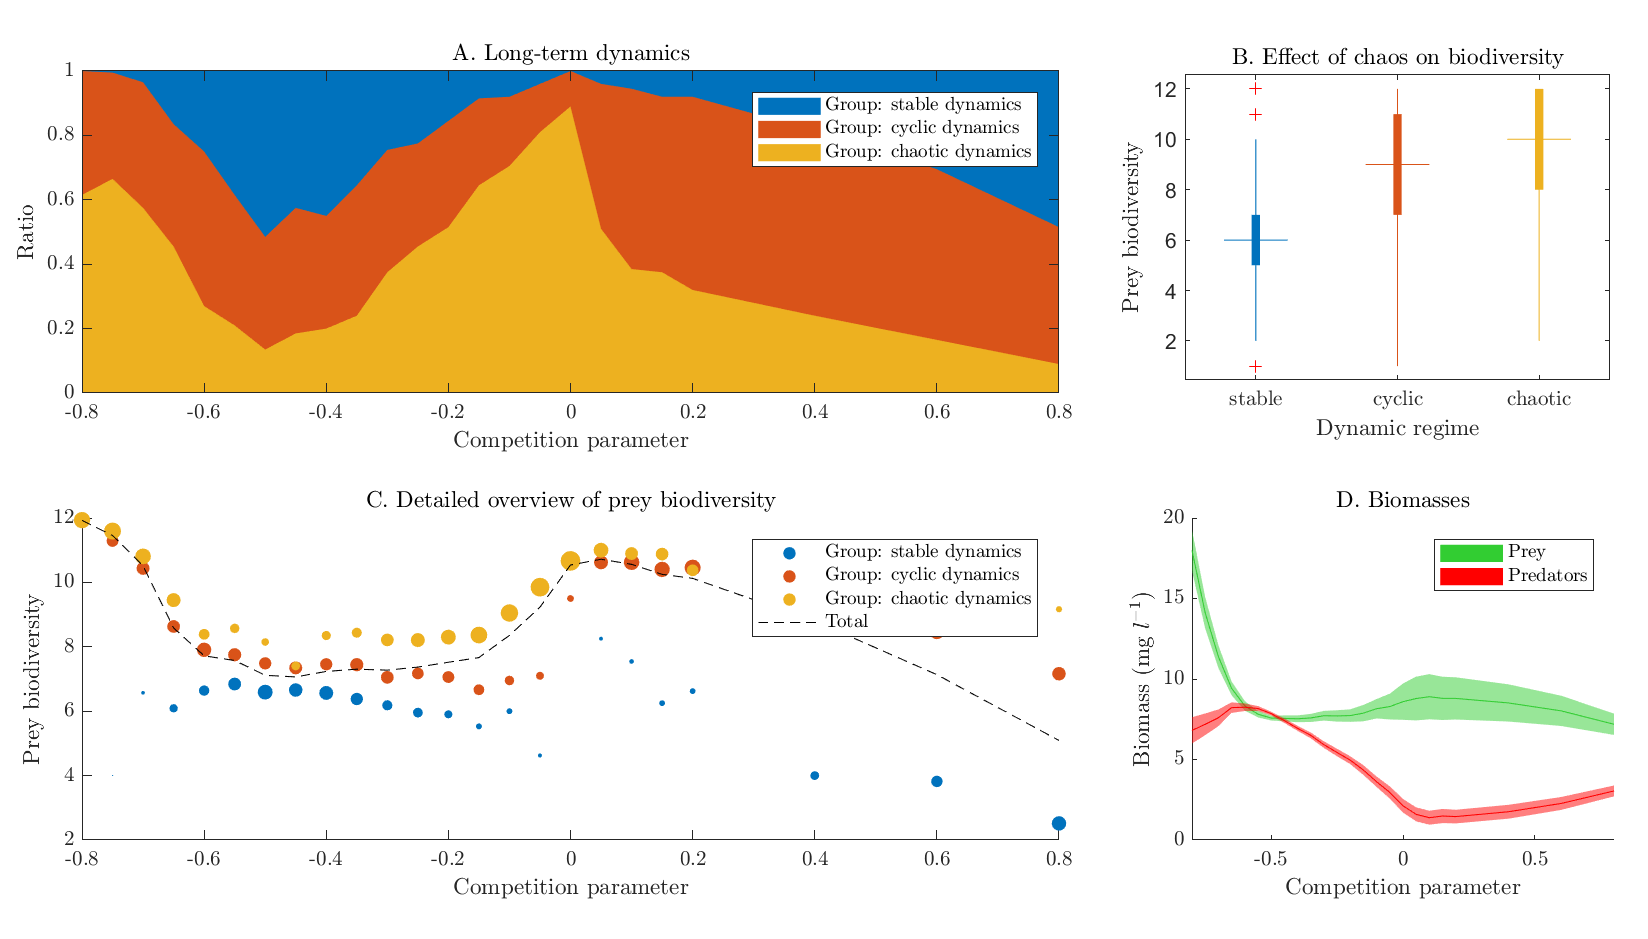
\includegraphics[width=1\columnwidth]{best.png}
	\end{center}
	\caption{Results for food webs with $8$ predator and $12$ prey species. Food webs of different sizes show similar results (see section \ref{subsec:GeneralResults} in Online Appendix). \textbf{Panel A}. Fraction of each dynamic regime as function of competition parameter ($n = \numReps$). \textbf{Panel B}. Box and whisker plot of the average number of non-extinct prey species grouped by asymptotic regime. \textbf{Panel C}. Average prey biodiversity as function of. competition parameter. The dashed line shows the average number of non-extinct prey species grouped by competition parameter. The colored circles represent the average prey biodiversity of the simulations, additionally grouped by dynamical regime (stable, cyclic and chaotic). The relative size of the circles represents the ratio of simulations that led to each kind of dynamics. \textbf{Panel D}. Average biomasses grouped by trophic level vs. competition parameter. The width represents standard deviation.}
	\label{fig:Biodiversity}
\end{figure}
